\chapter{شبیه‌سازی}
\noindent
\textbf{
	\textit{
		توصیف روند شبیه‌سازی سخت‌افزار و گام‌های اجرایی، مشاهدهٔ ورودی‌ها و خروجی‌های اصلی و میانی، مقایسه با مقادیر حاصل از اجرای کد نرم‌افزاری (مدل طلایی)، توصیف مراحل اجزای الگوریتم به همراه شکل موج‌ها، نحوهٔ عملکرد 
		\lr{Testbench}
	}
}
\pagebreak

\section{توضیح روند شبیه‌سازی سخت‌افزار و گام‌های اجرایی}
برای شبیه‌سازی سخت‌افزاری کد 
\lr{verilog}
الگوریتم 
\lr{Skein}
را در محیط شبیه‌سازی 
\lr{Modelsim}
اجرا کردیم. گام‌های اجرایی به صورت کلی برای شبیه‌سازی کد سخت‌افزاری موارد زیر بود. 
\begin{itemize}
	\item
	      مطالعه کد الگوریتم و تعیین ورودی‌ها
	\item
	      نوشتن Testbench
	\item
	      اجرای کد در محیط Modelsim با Testbench های مختلف
	\item
	      گرفتن Waveform و مقادیر خروجی (اصلی و میانی)
\end{itemize}
\section{مشاهدهٔ ورودی‌ها و خروجی‌های اصلی و میانی}
در ادامه ابتدا کد های Testbench اجرا شده بر الگوریتم و سپس Waveform
های حاصله و در انتها خروجی‌ها به صورت متنی آورده می‌شود.

\subsection{توضیح نحوهٔ عملکرد Testbench}
در ادامه ابتدا کد verilog نوشته‌شده برای  Testbench آورده  و سپس توضیحاتی دربارهٔ آن ایراد شده است. 
\pagebreak
\subsubsection{\lr{Testbench 1}}
\begin{code}
	//Master Testbench example
	
	module skein_tb;
	
	// Inputs
	reg clk;
	reg [511:0] midstate;
	reg [95:0] data;
	reg [31:0] nonce;
	
	// Outputs
	wire [511:0] hash;
	
	// Instantiate the Unit Under Test (UUT)
	skein512 uut (
	.clk(clk), 
	.midstate(midstate), 
	.data(data), 
	.nonce(nonce), 
	.hash(hash)
	);
	
	initial begin
	// Initialize Inputs
	clk = 0;
	midstate = 0;
	data = 0;
	nonce = 0;
	
	// Wait 100 ns for global reset to finish
	#1000
	data = 512'd12345609823;
	midstate = 96'd456;
	nonce = 32'd453;
	#1000;    
	data = 512'd7659432094555543122297600000000654;
	midstate = 96'd456;
	nonce = 32'd453;
	
	end
	always 
	#1 clk = ~clk;
	endmodule
\end{code}


\subsection{شکل موج حاصل از Testbench}

\subsubsection{\lr{Waveform 1}}
\begin{figure}[H]
	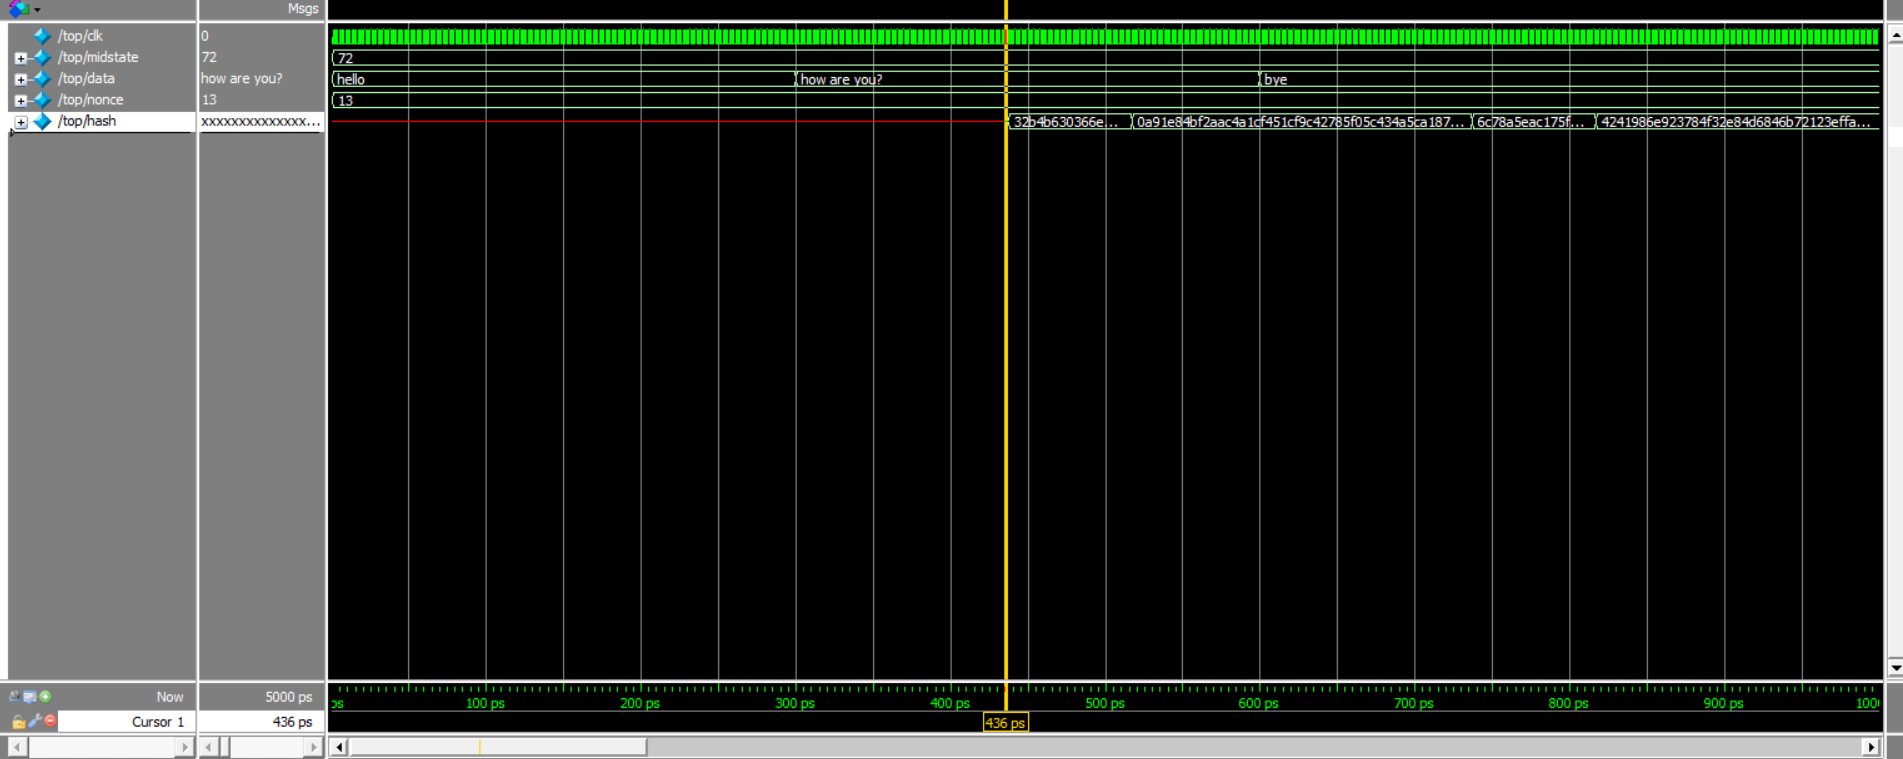
\includegraphics[width = \textwidth]{figs/simulation/1.png}
	\caption{شبیه‌سازی با \lr{Testbench}}
	\label{simulation_1}
\end{figure}

\subsection{جدول ورودی‌ها و خروجی‌های  Testbench}
\lr{
	\begin{table}[H]
		\resizebox{\textwidth}{!}{%
			\begin{tabular}{@{}llll@{}}
				\toprule
				Midstate & Nonce   & Data                                    & Time (clk)  \\ \midrule
				0        & 0       & 0                                       & 1000 - 0    \\
				96'd456  & 32'd453 & 512'd12345609823                        & 2000 - 1000 \\
				96'd456  & 32'd453 & 512'd7659432094555543122297600000000654 & End - 2000  \\ \bottomrule
			\end{tabular}%
		}
		\rl{
			\caption{مقادیر ورودی‌ها و زمان }}
		\label{table_input}
	\end{table}}

\lr{
	\begin{table}[H]
		\resizebox{\textwidth}{!}{%
			\begin{tabular}{@{}ll@{}}
				\toprule
				Hash                                                                                        \\ \midrule
				\begin{tabular}[c]{@{}l@{}}ab5283d68df053ac62d053789d4b45b81a02c959d7cab97fc43451166351f117 \\ f949fe918475f762ba80567046338211461648316d4432e6c505edc3b5ee6ff5\end{tabular} & 1217 - 433        \\
				\begin{tabular}[c]{@{}l@{}}dd477bfb0f07e299560b050c7aedb947bad77571f9a7d886a06f197a55f7946b \\ 8a9cecbb948a5478380168f8bfaf8e6d7d828459564973272b18cdf99d0234f2\end{tabular} & 1436 - 1217       \\
				\begin{tabular}[c]{@{}l@{}}0c0dea4dfd9994c6eb97f500589565239347be8a5b2e4ce4832c6cc9095baa51 \\ bf2bdde45ef619f4086e71e7d86f637314357e6d20632c31612f5424644cc223\end{tabular} & 2217 - 1436       \\
				\begin{tabular}[c]{@{}l@{}}6d383e0cceb223c20c45b816a165072ad200b8091682e8e5c31295ee62ca3719 \\ afbd493a4b85859d1cbe08d98bf01e66be18f3d3536987eeef06cc7965851bf8\end{tabular} & 2437 - 2217       \\
				\begin{tabular}[c]{@{}l@{}}6b722c1b1fb150c850e02ee44e03a447401ca4ac3cde4de6eb95b2e853d0d34b \\ 53583685f4b21f9b98229734756d7b835e46c2f589e461ab7c3177fb7e572b64\end{tabular} & End - 2437        \\ \bottomrule
			\end{tabular}%
		}
		\rl{
			\caption{مقادیر درهم‌سازی و زمان }}
		\label{table_hash}
	\end{table}}

